\documentclass[tikz,border=6pt]{standalone}
\usetikzlibrary{arrows.meta}
\begin{document}
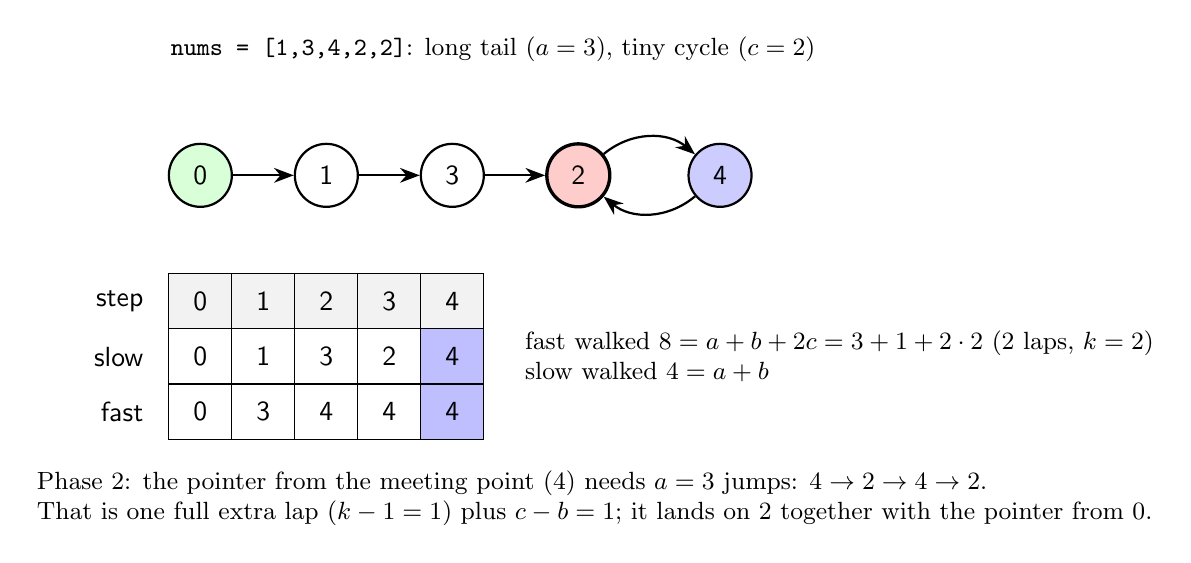
\begin{tikzpicture}[font=\sffamily,node_/.style={circle,draw,thick,minimum size=8mm},ar/.style={-{Stealth[length=2.5mm]},thick}]
\node[anchor=west,font=\small] at (-0.5,1.6) {\texttt{nums = [1,3,4,2,2]}: long tail ($a=3$), tiny cycle ($c=2$)};
\node[node_,fill=green!15] (n0) at (0,0) {0};
\node[node_] (n1) at (1.6,0) {1};
\node[node_] (n3) at (3.2,0) {3};
\node[node_,fill=red!20,very thick] (n2) at (4.8,0) {2};
\node[node_,fill=blue!20] (n4) at (6.6,0) {4};
\draw[ar] (n0)--(n1); \draw[ar] (n1)--(n3); \draw[ar] (n3)--(n2);
\draw[ar] (n2) to[bend left=40] (n4); \draw[ar] (n4) to[bend left=40] (n2);
\begin{scope}[yshift=-1.6cm,cell/.style={draw,minimum width=8mm,minimum height=7mm}]
\node[anchor=east] at (-0.6,0) {step}; \node[anchor=east] at (-0.6,-0.7) {slow}; \node[anchor=east] at (-0.6,-1.4) {fast};
\foreach \s/\f [count=\t from 0] in {0/0,1/3,3/4,2/4,4/4} { \node[cell,fill=gray!10] at (\t*0.8,0) {\t}; \node[cell] at (\t*0.8,-0.7) {\s}; \node[cell] at (\t*0.8,-1.4) {\f}; }
\node[cell,fill=blue!25] at (3.2,-0.7) {4}; \node[cell,fill=blue!25] at (3.2,-1.4) {4};
\node[anchor=west,font=\small,align=left] at (4.0,-0.7) {fast walked $8 = a + b + 2c = 3+1+2\cdot2$ (2 laps, $k=2$)\\slow walked $4 = a+b$};
\node[anchor=west,font=\small,align=left] at (-2.2,-2.5) {Phase 2: the pointer from the meeting point (4) needs $a=3$ jumps: $4\to2\to4\to2$.\\That is one full extra lap ($k-1=1$) plus $c-b=1$; it lands on 2 together with the pointer from 0.};
\end{scope}
\end{tikzpicture}
\end{document}
